% Options for packages loaded elsewhere
\PassOptionsToPackage{unicode}{hyperref}
\PassOptionsToPackage{hyphens}{url}
%
\documentclass[
  12pt,
]{article}
\usepackage{amsmath,amssymb}
\usepackage{iftex}
\ifPDFTeX
  \usepackage[T1]{fontenc}
  \usepackage[utf8]{inputenc}
  \usepackage{textcomp} % provide euro and other symbols
\else % if luatex or xetex
  \usepackage{unicode-math} % this also loads fontspec
  \defaultfontfeatures{Scale=MatchLowercase}
  \defaultfontfeatures[\rmfamily]{Ligatures=TeX,Scale=1}
\fi
\usepackage{lmodern}
\ifPDFTeX\else
  % xetex/luatex font selection
\fi
% Use upquote if available, for straight quotes in verbatim environments
\IfFileExists{upquote.sty}{\usepackage{upquote}}{}
\IfFileExists{microtype.sty}{% use microtype if available
  \usepackage[]{microtype}
  \UseMicrotypeSet[protrusion]{basicmath} % disable protrusion for tt fonts
}{}
\makeatletter
\@ifundefined{KOMAClassName}{% if non-KOMA class
  \IfFileExists{parskip.sty}{%
    \usepackage{parskip}
  }{% else
    \setlength{\parindent}{0pt}
    \setlength{\parskip}{6pt plus 2pt minus 1pt}}
}{% if KOMA class
  \KOMAoptions{parskip=half}}
\makeatother
\usepackage{xcolor}
\usepackage[margin=1in]{geometry}
\usepackage{graphicx}
\makeatletter
\def\maxwidth{\ifdim\Gin@nat@width>\linewidth\linewidth\else\Gin@nat@width\fi}
\def\maxheight{\ifdim\Gin@nat@height>\textheight\textheight\else\Gin@nat@height\fi}
\makeatother
% Scale images if necessary, so that they will not overflow the page
% margins by default, and it is still possible to overwrite the defaults
% using explicit options in \includegraphics[width, height, ...]{}
\setkeys{Gin}{width=\maxwidth,height=\maxheight,keepaspectratio}
% Set default figure placement to htbp
\makeatletter
\def\fps@figure{htbp}
\makeatother
\setlength{\emergencystretch}{3em} % prevent overfull lines
\providecommand{\tightlist}{%
  \setlength{\itemsep}{0pt}\setlength{\parskip}{0pt}}
\setcounter{secnumdepth}{5}
\usepackage{setspace} \usepackage{amsmath} \usepackage{array} \usepackage{caption} \usepackage{longtable} \usepackage{booktabs} \usepackage{enumitem} \renewcommand{\arraystretch}{1} \captionsetup[table]{skip=5pt} \setstretch{1.5}
\ifLuaTeX
  \usepackage{selnolig}  % disable illegal ligatures
\fi
\usepackage[]{natbib}
\bibliographystyle{apalike}
\IfFileExists{bookmark.sty}{\usepackage{bookmark}}{\usepackage{hyperref}}
\IfFileExists{xurl.sty}{\usepackage{xurl}}{} % add URL line breaks if available
\urlstyle{same}
\hypersetup{
  pdftitle={Attentional Discounted Utility},
  pdfauthor={Zijian Zark Wang},
  hidelinks,
  pdfcreator={LaTeX via pandoc}}

\title{Attentional Discounted Utility}
\author{Zijian Zark Wang}
\date{July 13, 2023}

\begin{document}
\maketitle

\hypertarget{introduction}{%
\section{Introduction}\label{introduction}}

\hypertarget{the-model}{%
\section{The Model}\label{the-model}}

\hypertarget{the-decision-process}{%
\subsection{The Decision Process}\label{the-decision-process}}

Suppose time is discrete. Let \(X_T\) denote the sequence of rewards
\([x_0,x_1,...,x_T]\), which yields reward \(x_t\) in time period
\(t\).\footnote{I use uppercase letters to represent a sequence and
  lowercase letters to represent elements within the sequence.} The time
length of this sequence, denoted by \(T\), is finite. For any
\(t \in \{0,1,...,T\}\), the reward level \(x_t\) is a random variable
defined on \(\mathbb{R}_{\geq 0}\). I assume that making an
intertemporal choice involves three steps:

\begin{itemize}[leftmargin=2cm]
\item[Step 1.] (\textit{Sampling}) The decision maker subjectively draws a few potential realizations of $X_T$, and from each drawn realization, she draws a few time periods and observes their rewards; then, she combines all observed rewards into a sample.

\item[Step 2.] (\textit{Valuation}) The decision maker uses the mean utility of sampled rewards as an approximate value representation of $X_T$.

\item[Step 3.] (\textit{Choice-making}) She chooses the sequence with the highest value from all the available reward sequences.
\end{itemize}

In the decision process described above, Step 3 is standard. By Step
1-2, I take the notion that, to evaluate a stimuli, the decision maker
needs to assess all the relevant information, while her information
processing capacity is limited. Consequently, she selectively attends to
only \emph{a subset} of the available information (which is termed
\emph{a sample}), then aggregates the attributes observed in the sample
to calculate the stimuli value. This sampling process is not unbiased;
on the contrary, the decision maker aims to retain more of the
information that they consider more relevant in the sample. Such a
notion has a long history in psychological research.\footnote{\citet{weber_mindful_2009}
  and \citet{chun_taxonomy_2011} provide good reviews for such studies.}
In recent years, many theories grounded in this (or similar notions)
have made significant progress in explaining choice anomalies, such as
decision field theory \citep{busemeyer_decision_1993},
decision-by-sampling \citep{stewart_decision_2006}, utility-weighted
sampling \citep{lieder_overrepresentation_2018} and efficient coding
theory \citep{heng_efficient_2020}. In the next subsection, I describe
the sampling and valuation process in detail.

\hypertarget{attention-mechanism-and-optimal-discounting}{%
\subsection{Attention Mechanism and Optimal
Discounting}\label{attention-mechanism-and-optimal-discounting}}

Let \(S_T=[s_0,s_1,...,s_T]\) be a potential realization of \(X_T\), and
\(\mathcal{S}(X_T)\) be the support of \(X_T\), i.e.~the smallest set
containing any potentially realized sequence \(S_T\), where
\(\mathcal{S}(X_T)\subseteq \mathbb{R}_{\geq 0}^{T+1}\). Let \(w(s_t)\)
be the probability that the reward of the \(t\)-th period in \(S_T\) is
in the sample, \(u(s_t)\) be the utility obtained by reward \(s_t\)
(\(t \in \{0,1,...,T\}\)), where \(u'>0\), \(u''<0\). The function
\(w(.)\) and \(u(.)\) are termed as weight function and instantaneous
utility function respectively. The approximate value of \(X_T\), which I
term by \(U(X_T)\), is calculated by
\(U(X_T)=\sum_{S_T\in \mathcal{S}(X_T)}\sum_{t=0}^T w(s_t) u(s_t)\).

The sampling process is sequential. At the very beginning, the decision
maker has no information about which period in a potentially realized
sequence \(S_T\) has a larger reward. After each sampling, she acquires
new information in this regard, and adjusts the sampling weights for
different time periods based on such information. Sampling and
processing information require mental effort from the decision maker,
thus trigger a cost \(C\) at the cognitive level. I assume the decision
maker's objective in this process is to find a sampling strategy,
denoted by weight function \(w(.)\), that can maximize the approximate
value of the given reward sequence (hereafter referred as ``overall
utility'') minus the cost of information, i.e.~maximizing \(U(X_T)-C\).
As the decision maker pays a higher cost in sampling as well as
processing information, these sampling weights will change in a way that
increases the overall utility. Therefore, we consider the cognitive cost
\(C\) as a functional of weight function \(w(.)\).

The problem of determining the weight function under the above setting
is termed as the constrained optimal discounting problem in Noor and
Takeoka
\citetext{\citeyear{noor_optimal_2022}; \citeyear{noor_constrained_2023}}.
I follow their terminology.

\textbf{Definition 1}: Let \(W\) be the smallest set containing all
possible weight functions. Given a stochastic reward sequence \(X_T\),
the following optimization problem is called the \emph{constrained
optimal discounting} problem for \(X_T\):\[ 
\begin{aligned}
\max_{w\in W}  \quad & \sum_{S_T\in \mathcal{S}(X_T)}\sum_{t=0}^T w(s_t)u(s_t) - C(w) \\
s.t. \quad &  \sum_{S_T\in \mathcal{S}}\sum_{t=0}^T w(s_t)=1 \\
& w(s_t)\geq 0, \forall t\in\{0,1,…,T\} \\
\end{aligned}
\]where \(C:[0,1]^{T+1}\rightarrow \mathbb{R}_{>0}\) is called a
\emph{information cost} function, \(\partial C/\partial w(s_t)>0\) and
\(\partial^2 C/\partial w(s_t)^2>0\). That is, the cost of information
is increasing and convex in \(w(s_t)\).

The assumption that \(C(.)\) is a convex function ensures the
constrained optimal discounting problem has an interior solution.
Notably, the objective function in Definition 1 implies that the
decision maker tends to pay a cost to make any period or state with a
larger reward be sampled more frequently. There are two reasons for
using this objective function. First, there is substantial evidence
indicating that people selectively attend to desirable information and
avoid unpleasant information.\footnote{This includes a wide range of
  behavioral biases, e.g.~ostrich effect, confirmation bias. For
  additional evidence, see \citet{golman_information_2017}.} For
instance, it is found investors are more likely to check their brokerage
accounts when stock market goes up \citep{sicherman_financial_2016}. In
the intertemporal choice setting, this suggests that the periods or
states with more desirable outcomes may receive more attention. Second,
as is pointed out in \citet{lieder_overrepresentation_2018}, the
sampling algorithm in the brain may share certain principles with
optimal importance sampling. In importance sampling, to minimize the
variance, the events with greater absolute utilities should be assigned
more importance, i.e.~being sampled with a higher probability. If the
same principle is applicable to the brain, it also provides a rationale
to this specific objective function.

After determining the weight function, the decision maker calculates the
overall utility that she can obtain from a reward sequence. Let
\(p(S_T)\) be the probability of \(S_T\) being sampled in the brain. I
define \(w_t(S_T) = \frac{w(s_t)}{p(S_T)}\). Thus, the overall utility
of \(X_T\) can be calculated using the expected discounted utility (EDU)
framework, i.e.~\(U(X_T)=E_p[\sum_{t=0}^Tw_t(S_t)u(s_t)]\). Under EDU
framework, the \(w_t(S_T)\) in braces is commonly referred to as the
\emph{discounting factor} for period \(t\) in \(S_T\), a certain
realization of sequence \(X_T\). Given that attentional mechanism plays
a prominent role in the valuation of \(X_T\), I call any \(U(X_T)\)
calculated in this way the \emph{attentional discounted utility}. When
each alternative sequence has been valuated, I assume the decision maker
will choose the sequence with highest attentional discounted utility
(ADU). This is shown in Definition 2.

\textbf{Definition 2}: For any sequence of rewards \(X_T\), \(X'_{T'}\),
preference relation \(\succsim\) has an \emph{attentional discounted
utility} (ADU) representation if and only if\[
X_T \succsim X'_{T'} \Longleftrightarrow U(X_T)\geq U(X'_{T'})
\]and \[
U(X_T)=\sum_{S_T\in\mathcal{S}(X_T)}\sum_{t=0}^T w(s_t)u(s_t),\quad 
U(X'_{T'})=\sum_{S_{T'}\in\mathcal{S}(X'_{T'})}\sum_{t=0}^{T'} w'(s_t)u(s_t)
\]where \(S_\tau\) denotes \([s_0, s_1,…, s_\tau]\), \(\tau\) is the
time length of \(S_\tau\), \(w(.)\) and \(w'(.)\) are the solutions to
constrained optimal discounting problems for \(X_T\) and \(X'_{T'}\).

\hypertarget{adu-with-shannon-cost-function}{%
\subsection{ADU with Shannon Cost
Function}\label{adu-with-shannon-cost-function}}

Hereafter I focus on a well-known specification of information cost
function, which I term Shannon cost function, proposed by
\citet{matejka_rational_2015}. The Shannon cost function was originally
used to justify the multinominal logit model in discrete choice
analysis, and so far has been topical in rational inattention
literature. To construct this style of information cost function,
\citet{matejka_rational_2015} introduce two assumptions. The first
assumption is, before acquiring any information, the decision maker
estiablishes an initial allocation of weights for different attributes,
which remains invariant over states. The weights are then updated in a
manner consistent with Bayes rule. Suppose the initial weight assigned
to period \(t\) is \(d_t\), then
\(d_t=\sum_{S_T\in \mathcal{S}(X_T)} w(s_t)\). The second assumption is,
the cost of information is linear to the information gains, measured by
Shannon mutual information. That
is,\[ C(w)= \lambda \sum_{S_T\in \mathcal{S}(X_T)}\sum_{t=0}^T w(s_t) \log\left(\frac{w_t(S_T)}{d_t}\right) \]where
\(\lambda\) is a parameter denoting unit cost of information
(\(\lambda>0\)). With the Shannon cost function, the constrained optimal
discounting problem can be easily solved by Lagrangian
method.\footnote{For how to solve this optimization problem, see
  \citet{matejka_rational_2015} or \citet{mackowiak_rational_2023}.} In
its solution, the discounting factor is calculated by
\[ w_t(S_T) =\frac{d_te^{u(s_t)/\lambda}}{\sum_{\tau=0}^T d_\tau e^{u(s_\tau)/\lambda}} \]

In this case, \(w_t(S_T)\) follows a logistic-like distribution. It is
increasing with \(u(x_t)\), indicating that the decision maker tends to
pay more attention to the periods with larger rewards; and is
``anchored'' in the initial weight \(d_t\), inidicating the adjustment
of attention allocation is costly. Meanwhile, note that the sum of
\(w_t(S_T)\) for any given \(S_T\) is fixed at 1, which implies the
decision maker's capacity of information processing is limited. If
Shannon cost function is used in determining weight function, I call the
overall utility calculated in the subsequent step as \emph{ADU with
Shannon cost function} (hereafter referred to as ADUS).

In a static choice setting, the rationale for the usage of Shannon cost
function can be interpreted with independence of irrelevant alternatives
\citep{matejka_rational_2015}, or data compression
\citep{caplin_rationally_2022}. However, this is not applicable when
weights can be allocated across time periods. Hence, I propose two
axioms that can characterize Shannon cost function in the intertemporal
choice setting.

\textbf{Axiom 1}: For any reward sequence \(X_T\), \(X'_T\), \(X''_T\)
and \(\alpha\in(0,1)\), \(X_T\succ X'_T\) implies
\(\alpha X_T+ (1-\alpha)X''_T \succ \alpha X'_T + (1-\alpha) X''_T\).

Axiom 1 can be interpreted by Lemma 1.\footnote{The preference relation
  \(x \succ y\) is defined by the opposite of \(y\succsim x\); the
  preference relation \(x\sim y\) is defined by the joint satisfaction
  of \(x\succsim y\) and \(y \succsim x\).}

\textbf{Lemma 1}: (\emph{state independence}) Suppose preference
relation \(\succsim\) has an ADU representation and satisfies Axiom 1.
If \(p_1+p_2+...p_n=1\), and for any \(i\in\{1,2,…,n\}\), \(0<p_i<1\),
then for any deterministic reward sequence \(S^1_T\), \(S^2_T\), \ldots,
\(S^n_T\), we have\[
U(p_1 S^1_T+p_2S^2_T+...+p_nS^n_T)=p_1U(S^1_T)+p_2U(S^2_T)+...+p_nU(S^n_T)
\]Lemma 1 implies that, the determination of discounting factors for one
potential realization of a reward sequence will not interfere with that
for another potential realization of it. Suppose \(S_T\) and \(S'_{T}\)
are both potential realizations of a reward sequence \(X_T\), one can
solve \(w_t(S_T)\) and \(w_t(S'_T)\) by constructing a constrained
optimal discounting problem for each then solving it independently.

\textbf{Axiom 2}: For any non-negative real number \(c\) and
deterministic reward sequence \(S_T\), let \(cS_T\) denote
\([c,s_0,s_1,...,s_T]\), there always exists \(\alpha\in(0,1)\) such
that \(cS_T\sim (1-\alpha)c+\alpha S_T\).

Axiom 2 can be interpreted by Lemma 2.

\textbf{Lemma 2}: (\emph{spread-consistency correlation}) Suppose
preference relation \(\succsim\) has an ADU representation and satisfies
Axiom 2. If there exist \(c\) and \(S_T\) such that, for any \(c'\) and
\(S_T'\), \(cS_T\succsim c'S_T'\), where
\(c+\sum_{t=0}^Ts_t=c'+\sum_{t=0}^Ts_t'\), then for any \(S'_T\), we
have \[S_T \succsim S_T' \Longleftrightarrow c\sim S_T\]where
\(\sum_{t=0}^Ts_t=\sum_{t=0}^Ts_t'\).

Lemma 2 implies that, when allocating a consumption budget across time
periods, the decision maker keeps her choice dynamically consistent if
and only if she performs a strong preference for spread. Given that
people are typically assumed to be impatient (preferring a declining
sequence), one intuitive interpretation of Lemma 2 is that the less
impatient a decision maker is in the present, the less inclined she is
to deviate from the original choice in the future.

\textbf{Proposition 1}: \(\succsim\) \emph{has an ADUS representation if
and only if it has an ADU representation and satisfies Axiom 1-2.}

\hypertarget{implications-in-time-preferences}{%
\section{\texorpdfstring{Implications in Time Preferences
\label{behavioral}}{Implications in Time Preferences }}\label{implications-in-time-preferences}}

To illustrate how ADU with Shannon cost function can account for a broad
set of anomalies about time preferences, imagine that a decision maker
receives a positive detereminstic reward in period \(j\) (and no reward
in other periods). That is, she receives a sequence of rewards
\(X_T=[x_0,x_1,…,x_T]\), where \(x_j>0\) and is certain, and \(x_t = 0\)
for all \(t \neq j\) (both \(j\) and \(t\) are in \(\{0,1,...,T\}\)).

For the convenience of illustration, I assume the decision maker holds
stationary time preferences before acquiring any information, that is,
\(d_t=\delta^t\). Meanwhile, \(\delta\in(0,1]\), where \(\delta=1\)
implies the initial attention is uniformly distributed across periods.
For simplicity, I define \(v(x_t)=u(x_t)/\lambda\), and set \(v(0)=0\).
Let \(w_t(X_T)\) denote the discounting factor for period \(t\). From
the formula of ADUS we can infer that\[ 
w_j(X_T) = \left\{ \begin{aligned}
& \delta^j \cdot\frac{1}{1+\frac{\delta}{1-\delta}(1-\delta^T)e^{-v(x_j)}}\;, & 0<\delta<1 \\
& \frac{1}{1+T\cdot e^{-v(x_j)}}\; , & \delta=1
\end{aligned}
\right.
\]

Clearly, \(w_j\) is decreasing in \(T\). This offers an account for a
phenomenon called \emph{hidden zero effect}.

\hypertarget{hidden-zero-effect}{%
\subsection{Hidden Zero Effect}\label{hidden-zero-effect}}

The most direct evidence that could support the ADUS model is likely the
hidden zero effect \citep{magen_hidden-zero_2008}. The hidden zero
effect means, supposing people face a small sooner reward (SS) and a
large later reward (LL), they tend to exhibit more patience when SS and
LL are framed as sequences rather than being framed as single-period
rewards. For instance, suppose SS is ``receive £100 today'' and LL is
``receive £120 in 6 months'', and we have

SS\textsubscript{0}: ``receive £100 today and £0 in 6 months''

LL\textsubscript{0}: ``receive £0 today and £120 in 6 months''

people will be more likely to prefer LL\textsubscript{0} over
SS\textsubscript{0} than preferring LL over SS. Subsequent research
(e.g. \citet{read_value_2017}) suggests that the hidden zero effect is
asymmetric. That is, shifting SS to SS\textsubscript{0} and keeping LL
unchanged leads to an increase in patience, whereas shifting LL to
LL\textsubscript{0} and keeping SS unchanged cannot increase patience.
ADUS assumes that, within a sequence, attention is limited and the
weight assigned to each period is anchored in an initial positive
weight. These properties naturally explain the hidden zero effect. To
illustrate, in SS, the decision maker perceives the length of sequence
as ``today'' and allocate no attention to future. Whereas, in
SS\textsubscript{0}, she perceives the length as ``6 months''. This
makes some attention be paid to future periods with no reward, and
decreases the attention paid to the only period with positive reward
(given attention is limited); thus, the overall utility of sequence
decreases. By contrast, shifting from LL to LL\textsubscript{0} does not
change the length of sequence, thus does not change overall utility.

The existence of hidden zero effect also provides a hint in selection of
time length \(T\). When evaluating a reward delivered in period \(j\),
the range of \(T\) is \([j,+\infty)\). Any increase in \(T\) will reduce
the overall utility. Thus, when comparing SS and LL, the decision maker
may tend to set \(T=j\) (the minimum length she can set), in order to
maximize the overall utility. Any period out of this length can be
perceived as irrelevant to the decision; so, she does not need to sample
from the periods after \(j\), when evaluating the given reward. Though,
explicitly mentioning the periods after \(j\) will direct her attention
to those periods, and lead to the hidden zero effect. By setting
\(T=j\), we
have\[ w_T(x_T) = \frac{1}{1+G(T)e^{-v(x_T)}} \]where\[ G(T) = \left\{ \begin{aligned} & \frac{1}{1-\delta}(\delta^{-T}-1) \; ,& 0<\delta<1\\ & T\; ,& \delta=1\ \end{aligned} \right. \]

Given period \(T\) is now the only period with a non-zero reward within
the sequence, I use \(x_T\) to directly represent the whole sequence,
and let \(w_T(x_T)\) denote the discounting factor for period \(T\).
Interestingly, when \(\delta=1\), \(w_T(x_T)\) takes a form similar with
hyperbolic discounting.

\hypertarget{common-difference-effect}{%
\subsection{Common Difference Effect}\label{common-difference-effect}}

A well-known anomaly about time preferences is \emph{common difference
effect}, firstly defined by \citet{loewenstein_anomalies_1992}. Suppose
there are a large later reward \(x_l\) arriving at period \(t_l\)
(denoted by LL) and a small sooner reward \(x_s\) arriving at period
\(t_s\) (denoted by SS), where \(x_l>x_s>0\), \(t_l>t_s>0\). Define
\(V(x,t)=w_t(x_t)v(x_t)\). The common difference effect means,
supposing\(V(x_l,t_l)=V(x_s,t_l)\), we must have
\(V(x_l,t_l+\Delta t)>V(x_s,t_s+\Delta t)\) for any positive integer
\(\Delta t\).

ADUS predicts that, if people are impatient, to observe the common
difference effect, the difference between SS and LL in reward level must
be set significantly larger than the difference in time delay. This is
shown in Proposition 2.

\textbf{Proposition 2}: \emph{In ADUS, if the initial weights are
uniformly distributed, then the common difference effect always holds;
if the initial weights exponentially declines over time, the common
difference effect holds when}
\(v(x_l)-v(x_s)+\ln\frac{v(x_l)}{v(x_s)}>-(t_l-t_s)\ln\delta\)\emph{.}

Proposition 2 is interpreted as follows. When \(\delta = 1\), ADUS
predicts the decision maker always performs the common difference
effect. This is obvious because discounting factor \(w_T(x_T)\) takes a
hyperbolic-like form. When \(\delta<1\), there are four factors jointly
deciding whether we could observe the common difference effect or not.
First, without considering attentional mechanism, when we extend time
delay, each of \(w_{t_l}(x_l)\) and \(w_{t_s}(x_s)\), i.e.~the
discounting factor for (and attention paid to) the only period with
positive reward, declines in an exponential fashion. Second, without
considering newly added time interval, due to the decline of
\(w_{t_l}(x_l)\) and \(w_{t_s}(x_s)\), the decision maker frees up some
attention and can reallocate it across periods. Given that in LL, the
decision maker has to wait longer for reward, the periods where she wait
can grab more attention from the released capacity of attention,
compared with those in SS. In other words, an extension of delay makes
she focus more on the waiting time in LL than in SS, which decreases the
preference for LL. Third, the newly added time interval also grabs some
attention from other periods. Note the time delay is extended by
\([t_l,t_l+\Delta t]\) in LL and by \([t_s, t_s+\Delta t]\) in SS; given
\(t_l>t_s\), if people are impatient, the newly added time interval will
receive less attention in LL than in SS, without considering other
factors. This increases the preference for LL. Fourth, ADU generally
assumes that the decision maker tends to pay more attention to periods
with larger rewards. Given \(x_l>x_s\), the newly added interval grabs
less attention from the period where \(x_l\) is positioned (in LL) than
from the period where \(x_s\) is positioned (in SS). That is, the
decision maker focuses comparatively more on reward level in LL than in
SS, which mitigates the impact of discounting factor declining. This
also increases the preference for LL. When the impact of the later two
factors succeeds that of the second factor, the decision maker will
perform the common difference effect.

Notably, if we explicit mention the zeros in LL and SS, extending time
delay always lead to the common difference effect.

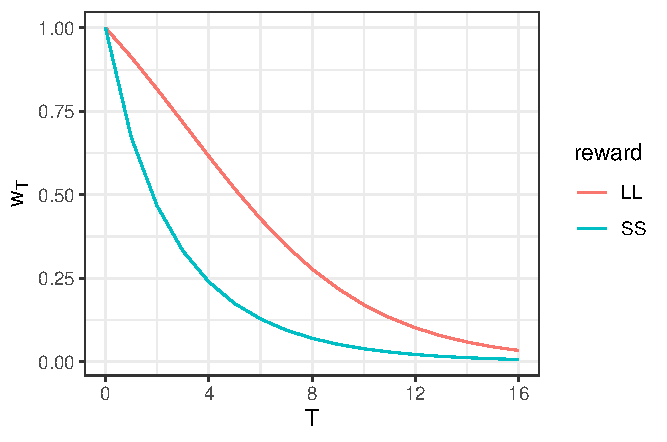
\includegraphics{images/weight_LLvSS.pdf}

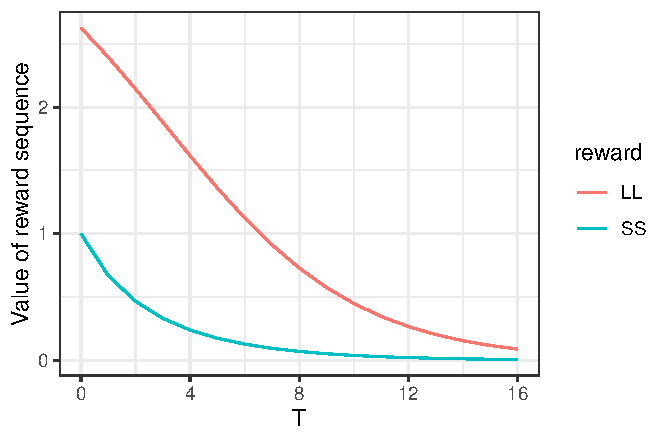
\includegraphics{images/value_LLvSS.pdf}

\hypertarget{magnitude-effect}{%
\subsection{Magnitude Effect}\label{magnitude-effect}}

The \emph{magnitude effect} is another well-known anormaly about time
preferences. Assuming we have \(t_l\), \(t_s\), \(x_s\) fixed, and want
to find a \(x_l\) such that \(V(x_l,t_l) \equiv V(x_s,t_s)\), the
magnitude effect implies that, if we increase \(x_s\), then the
\(x_l/x_s\) that makes the equality valid will decrease.

In standard discounted utility model, the magnitude effect requires the
elasticity of utility function to increase with the reward level
\citep{loewenstein_anomalies_1992}. This requirement might be too
restrictive, so that many commonly used utility functions (such as power
or CARA utility function) does not satisfy it. By contrast, in ADU
model, decision maker is generally assumed to attend more to periods
with larger rewards. This implies that when comparing SS and LL, she
exhibits more patience towards larger reward level, which is naturally
compatible with the magnitude effect
\citep{noor_intertemporal_2011, noor_optimal_2022}. By Proposition 3, I
focus on ADU with Shannon cost function, and show how this requirement
for curvature of utility function can be relaxed in this setting.

\textbf{Proposition 3}: \emph{Define} \(v(x)\equiv u(x)/\lambda\)
\emph{as the utility function. In ADUS, the magnitude effect always
holds true when function} \(v(x)\) \emph{satisfies}\[
RRA_v(x)\leq 1-\frac{e_v(x)}{v(x)+1}
\]\emph{where} \(RRA_v(x)\) \emph{is the relative risk aversion
coefficient of} \(v(x)\)\emph{,} \(e_v(x)\) \emph{is the elasticity of}
\(v(x)\) \emph{to} \(x\)\emph{.}

Note that Proposition 3 is a very broad condition. In Corollary 1 and
Corollary 2, I show that power utility function and CARA utility
function both satisfy this condition in most cases.

\textbf{Corollary 1}: Suppose \(v(x)=x^\gamma/\lambda\), where
\(0<\gamma<1\) and \(\lambda>0\). Then magnitude effect holds true for
any \(x\in \mathbb{R}_{>0}\).

\textbf{Corollary 2}: Suppose \(v(x)=(1-e^{-\gamma x})/\lambda\), where
\(\gamma>0\) and \(\lambda>0\). The magnitude effect holds true for any
\(x\geq \frac{1+\eta}{\gamma}\), where \(\eta>0\) and
\(\eta e^{1+\eta}-\eta=1\) (it can be calculated that
\(\eta \approx 0.35\)).

\hypertarget{concavity-of-time-discounting}{%
\subsection{Concavity of Time
Discounting}\label{concavity-of-time-discounting}}

Many time discounting models assumes discount function is convex in time
delay, e.g.~exponential and hyperbolic discounting. This style of
discount function predicts decision maker is \emph{risk seeking over
time lotteries}. That is, suppose a deterministic reward of level \(x\)
is delivered in period \(t_l\) with probability \(\pi\) and delivered in
period \(t_s\) with probability \(1-\pi\) (\(0<\pi<1\), \(c>0\)); while
another deterministic reward, of the same level, is delivered in a
certain period \(t_m\), where \(t_m=\pi t_l +(1-\pi) t_s\). The decision
maker should prefer the former reward to the latter reward. However,
some experimental studies, such as \citet{onay_intertemporal_2007} and
\citet{dejarnette_time_2020}, suggest that people are often \emph{risk
averse over time lotteries}, i.e.~preferring the reward delivered in a
certain period.

One way to accommodate the evidence about risk aversion over time
lotteries, as is suggested by \citet{dejarnette_time_2020}, is to modify
the convexity (concavity) of discount function. Under a general EDU
framework, decision maker is risk averse over time lotteries when
\(\pi w_{t_l}(x)+(1-\pi)w_{t_s}(x)<w_{t_m}(x)\). Fixing \(t_s\) and
\(t_l\), the inequality suggests \(w_{t_m}(c)\) is concave in \(t_m\).
In reverse, being risk seeking over time lotteries suggests
\(w_{t_m}(x)\) is convex in \(t_m\). Notably,
\citet{onay_intertemporal_2007} find that people are more likely to be
risk averse over time lotteries when \(\pi\) is small, and to be risk
seeking over time lotteries when \(\pi\) is large. Given that when
\(\pi\) gets larger, \(t_m\) is also larger, we can conclude that the
discount function may be concave in delay for the near future but convex
for the far future. Moreover, \citet{takeuchi_non-parametric_2011} also
find evidence that support this shape of discount function.

In Proposition 4, I show that ADUS can produce such a shape of discount
function as long as the reward level \(x\) is large enough.

\textbf{Proposition 4}: In ADUS, \emph{if} \(\delta =1\)\emph{, then the
discount function is convex in} \(t\)\emph{. If} \(0<\delta<1\)\emph{,
then there are a reward threshold} \(\underline{x}\) \emph{and a time
threshold} \(\underline{t}\) \emph{such that}

\begin{enumerate}
\def\labelenumi{\arabic{enumi})}
\tightlist
\item
  \emph{when} \(x\leq \underline{x}\)\emph{, the discount function is
  convex in} \(t\)\emph{;}
\item
  \emph{when} \(x > \underline{x}\)\emph{, the discount function is
  convex in} \(t\) \emph{given} \(t\geq \underline{t}\)\emph{, and it is
  concave in} \(t\) \emph{given} \(t<\underline{t}\)\emph{.}
\end{enumerate}

\emph{It can be derived that}
\(v(\underline{x})=\ln(\frac{2}{1-\delta})\)\emph{, and}
\(\underline{t}=\frac{\ln[(1-\delta)e^{v(x)}-1]}{-\ln\delta}\)\emph{.}

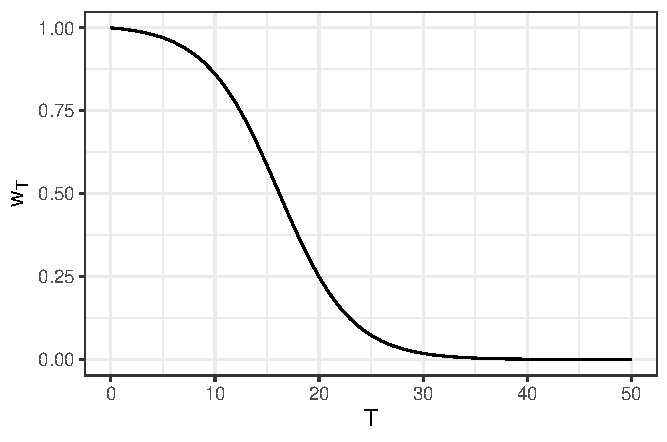
\includegraphics{images/concavity_discount.pdf}

\hypertarget{s-shaped-value-function}{%
\subsection{S-Shaped Value Function}\label{s-shaped-value-function}}

In prospect theory, \citet{kahneman_prospect_1979} propose an S-shaped
value function that is convex for losses and concave for gains. Since
that, S-shaped value functions have been widely embraced by behavioral
economists. More recent theories have provided further justifications
for it, including reference-dependent utility in a broad sense
\citep{koszegi_model_2006}, and efficient coding of values
\citep{frydman_efficient_2021}. Here, I provide an account based on
selective attention to time periods.

Suppose a decision maker is faced with a choice between a risky lottery
and a fixed amount of money. When making this choice, she does not
obtain any money from either option. Thus, she perceives the outcome of
each option as something that will happen in the future. She allocate
her attention between the present period and the period when she may
receive the money. Assume that she perceives the outcome will be
realized in period \(t\), and in a certain state, the option she chooses
yields reward \(x\), then we can use the attentional discounted utility
\(V(x,t)\) to represent the value function. I derive the conditions in
which ADUS can produce a S-shaped value function in Proposition 5.

\textbf{Proposition 5}: \emph{Suppose} \(t\geq1\)\emph{,}
\(\frac{d}{dx}\left(\frac{1}{v'(x)}\right)\) \emph{is continuous in}
\((0,+\infty)\)\emph{, in ADUS,}

\begin{enumerate}
\def\labelenumi{\arabic{enumi})}
\item
  \emph{there exists a threshold} \(\bar{x}\) \emph{in} \((0,+\infty)\)
  \emph{such that} \(V(x,t)\) \emph{is strictly concave in} \(x\)
  \emph{when} \(x\in [\bar{x},+\infty)\)\emph{;}
\item
  \emph{if} \(\frac{d}{dx}\left(\frac{1}{v'(x)}\right)\) \emph{is
  right-continuous at} \(x=0\)\emph{, and}
  \(\frac{d}{dx}\left(\frac{1}{v'(0)}\right)<1\)\emph{, then there
  exists a threshold} \(x^*\) \emph{in} \((0, \bar{x})\) \emph{such
  that, for any} \(x\in (0,x^*)\)\emph{,} \(V(x,t)\) \emph{is strictly
  convex in} \(x\)\emph{;}
\item
  \emph{there exist a hyper-parameter} \(\lambda^*\) \emph{and an
  interval} \((x_1,x_2)\) \emph{such that, if}
  \(\lambda<\lambda^*\)\emph{, for any} \(x\in(x_1,x_2)\)\emph{,}
  \(V(x,t)\) \emph{is strictly convex in} \(x\)\emph{, where}
  \(\lambda^*>0\) \emph{and} \((x_1,x_2)\subset(0,\bar{x})\)\emph{.}
\end{enumerate}

Proposition 5 implies, if the derivative of \(\frac{1}{v'(x)}\)
converges to a small number when \(x\rightarrow 0^+\), or the unit cost
of information \(\lambda\) is small enough, value function \(V(x,t)\)
will perform an S shape in some interval of \(x\). At the intuition
level, note that \(V(x,t)=w_t(x)v(x)\). When the level of reward \(x\)
grows, both the instantaneous utility of it, i.e.~\(v(x)\), and the
discounting factor assigned to it, i.e.~\(w_t(x)\), can increase. These
functions are both concave in \(x\): when the level of reward is small,
they both grow fast. So, it is possible that their product is convex in
this case. By contrast, when the level of reward is large, they grow
slowly, so their product keeps concave.

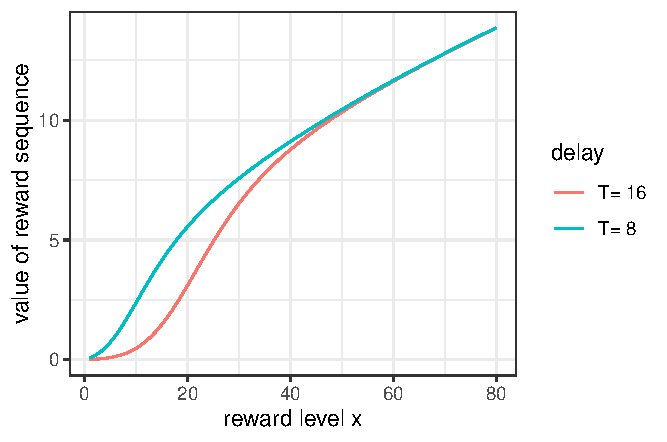
\includegraphics{images/S_shaped_value.pdf}

\hypertarget{inseparability-of-sequences}{%
\subsection{Inseparability of
Sequences}\label{inseparability-of-sequences}}

Let \(x\) and \(y\) denote two 2-period risky reward sequences. For
\(x\), the realized sequence is {[}£100,£100{]} with probability 1/2,
and is {[}£3,£3{]} with probability 1/2. For \(y\), the realized
sequence is {[}£3,£100{]} with probability 1/2, and is {[}£100,£3{]}
with probability 1/2. Classical models of intertemporal choice typically
assume the separability of potentially realized sequences. This implies
that the decision maker is indifferent between \(x\) and \(y\). However,
\citet{andersen_multiattribute_2018} find evidence of
\emph{intertemporal correlation aversion}, that is, people often prefer
\(y\) to \(x\).

ADU can naturally yield intertemporal correlation aversion. For
simplicity, suppose the initial attention is uniformly distributed
across the two periods. For \(x\), under each potentially realized
sequence, the decision maker equally weights each period. For \(y\),
decision maker tends to assign more weight to the period with a reward
of £100 (suppose that weight is \(w\)). Then the value of \(x\) is
\(\frac{1}{2} u(100) + \frac{1}{2} u(3)\) and the value of \(y\) is
\(w\cdot u(100) +(1-w) \cdot u(3)\). Given that \(x>\frac{1}{2}\), the
decision makers should strictly prefer \(y\) to \(x\).

\begin{itemize}
\tightlist
\item
  Other evidence related to inseparability: common sequence effect,
  (reverse) mere token effect, magnitude-increasing temporal sensitivity
\end{itemize}

\hypertarget{the-role-of-attention-in-inconsistent-planning}{%
\section{The Role of Attention in Inconsistent
Planning}\label{the-role-of-attention-in-inconsistent-planning}}

\hypertarget{empirical-analysis}{%
\section{Empirical Analysis}\label{empirical-analysis}}

\hypertarget{discussion}{%
\section{Discussion}\label{discussion}}

\hypertarget{conclusion}{%
\section{Conclusion}\label{conclusion}}

\renewcommand\refname{Reference}
  \bibliography{reference.bib}

\end{document}
